\begin{enumerate}[label=\thesection.\arabic*.,ref=\thesection.\theenumi]
\numberwithin{equation}{enumi}
\numberwithin{figure}{enumi}
\item Using Nyquist criterion, find out whether the system below is stable or not

\begin{align}
    G(s)= \frac{41}{s^2(s+3)}
    \label{eq:ee18btech11041_1}
\end{align}

\begin{align}
    H(s)= (s+4)
    \label{eq:ee18btech11041_2}
\end{align}
\solution 
According to the Nyquist criteria the number of unstable closed-loop poles (Z) is equal to the number of unstable open-loop poles (P) plus the number of clockwise encirclements (N) of the point (-1,j0) of the Nyquist plot of G(s)H(s), i.e

\begin{align}
    Z=N+P
    \label{eq:ee18btech11041_3}
\end{align}

Open loop transfer function :
\begin{align}
    G(s)H(s)=\frac{41(s+4)}{s^2(s+3)}
    \label{eq:ee18btech11041_4}
\end{align}

Closed loop transfer function:

\begin{align}
   T(s)= \frac{G(s)}{1+G(s)H(s)}=\frac{41}{s^3+3s^2+41s+164}
\end{align}

\begin{figure}[!h]
    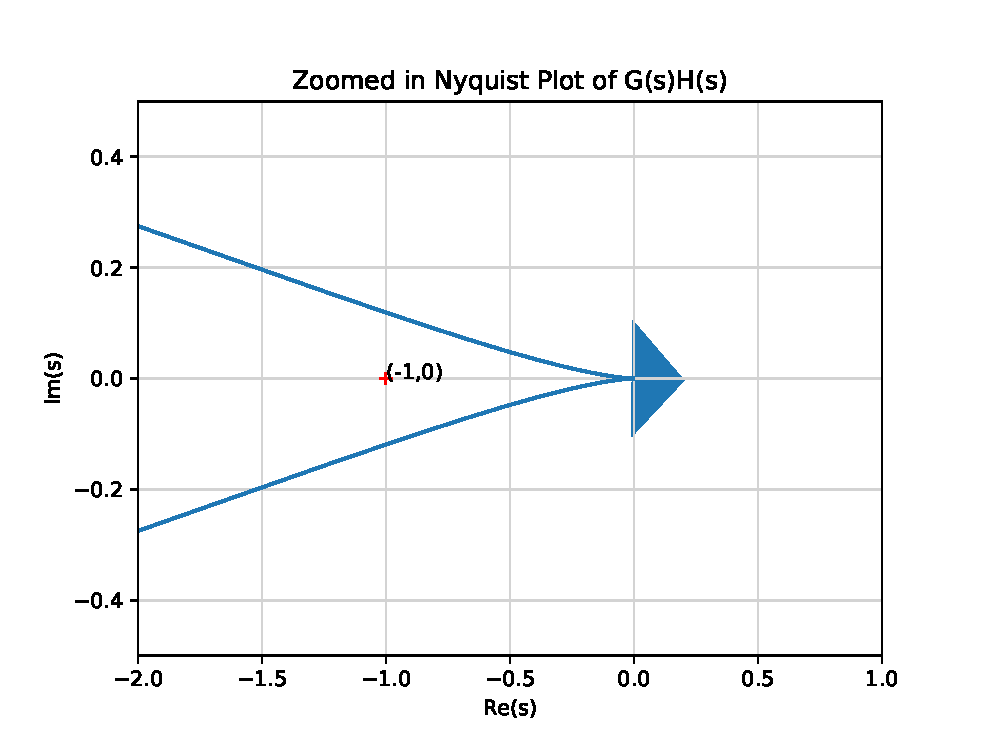
\includegraphics[width=\columnwidth]{./figs/ee18btech11041_1.eps}
    \caption{}
    \label{fig:1}
\end{figure}

\begin{figure}[!h]
    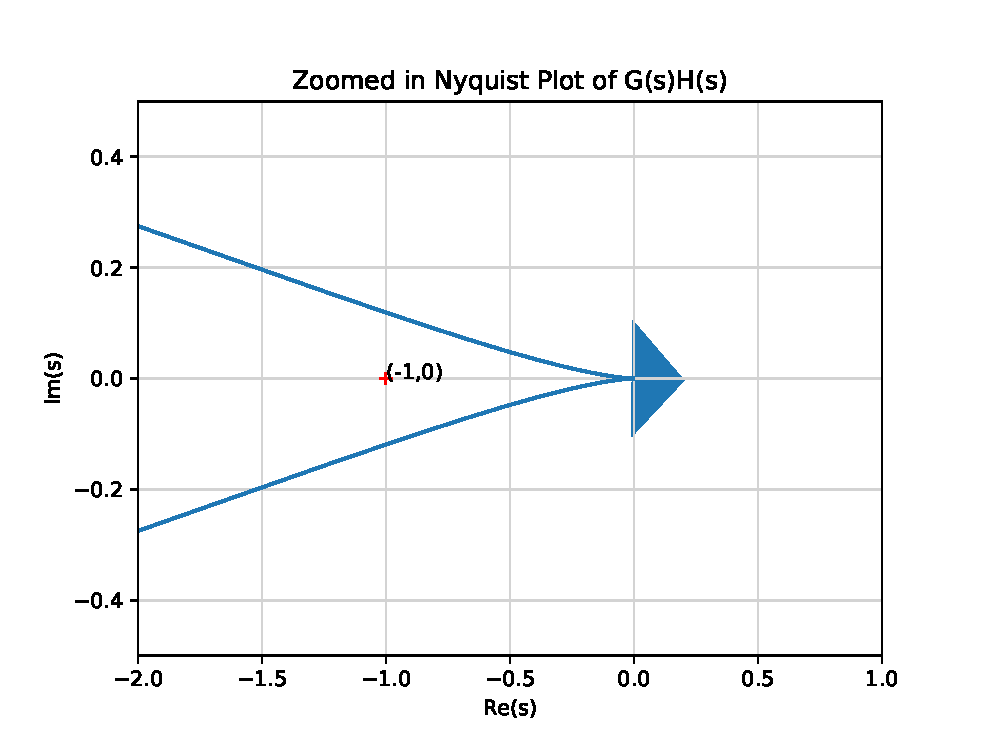
\includegraphics[width=\columnwidth]{./figs/ee18btech11041_2.eps}
    \caption{}
    \label{fig:2}
\end{figure}


In Fig.\ref{fig:2} it can be seen that there is a clockwise encirclement around (-1+0j).
As the open loop transfer function has zero pole of multiplicity 2, therefore it should be assumed that the phasor travels 2 times clock-wise along a semicircle of infinite radius Fig.\ref{fig:3} 

\begin{figure}[!h]
    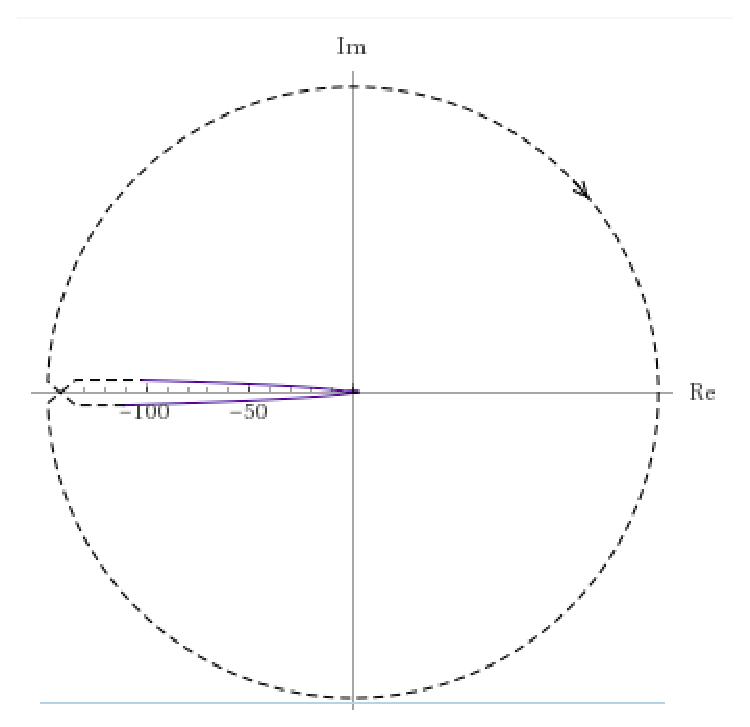
\includegraphics[width=\columnwidth]{./figs/ee18btech11041_3.eps}
    \caption{}
    \label{fig:3}
\end{figure}
\begin{center}
N=2, P=0    
\end{center}

\begin{align}
    \implies Z = 2
\end{align}

Therefore, The system T(s) is unstable as it has two poles on the right side of the s plane. 
The following code generates the nyquist plot
\begin{lstlisting}
codes/ee18btech11041.py
\end{lstlisting}


\end{enumerate}
